\documentclass[letterpaper]{article}
\usepackage[submission]{aaai2027}
\usepackage{times}
\usepackage{helvet}
\usepackage{courier}
\usepackage[hyphens]{url}
\usepackage{graphicx}
\usepackage{natbib}
\urlstyle{rm}
\def\UrlFont{\rm}
\usepackage{caption}
\frenchspacing
\setlength{\pdfpagewidth}{8.5in}
\setlength{\pdfpageheight}{11in}
\usepackage{amsmath}
\usepackage{amssymb}
\usepackage{amsthm}
\usepackage{booktabs}
\newtheorem{definition}{Definition}
\newtheorem{lemma}{Lemma}
\newtheorem{proposition}{Proposition}
\newtheorem{theorem}{Theorem}
\newtheorem{corollary}{Corollary}
\renewcommand{\qedsymbol}{}
\usepackage{multirow}
\usepackage{tikz}
\usepackage{placeins}
\usepackage{cuted}
\emergencystretch=1.2em
\usetikzlibrary{arrows.meta,positioning,calc,fit}
\pdfinfo{
/TemplateVersion (2026.1)
}
\setcounter{secnumdepth}{2}

\title{Affordable Real Style Transfer:\\Training Wavelet-Decoupled Rectified Flow on a Single RTX 3060 in Minutes}
\author{Anonymous Submission}
\affiliations{}
\begin{document}
\maketitle

\begin{abstract}
Art-to-art style transfer is easy to overclaim because the source image is already an artwork.
If the unchanged source already resembles the target domain, high style similarity can come from doing almost nothing.
We formalize this issue with identical-image transfer (IDT).
The unchanged source defines a no-op floor.
A method below that floor has not moved in the requested direction.

We then analyze why compact flow models often fall into this regime.
In Euclidean latent coordinates, low-frequency layout motion and high-frequency texture motion share one basis.
The flow objective can then favor structure preservation and suppress style-conditioned transport.
We state a sufficient local condition for this style-suppression regime and turn it into ablation-level predictions.

We propose \textnormal{WD-VF}, a wavelet-decoupled rectified flow in the latent space of the Stable Diffusion v1.5 EMA VAE.
A single-level Haar transform separates LL, LH, HL, and HH subbands.
WD-VF weakens LL supervision, routes style queries through high-frequency bands, and applies whitening and coloring only at the endpoint.
This keeps global structure stable while concentrating model capacity on stroke and texture transfer.

On Distinct5-WikiArt, the WD-VF model (with a trainable flow backbone of 903K parameters, excluding the frozen VAE) reaches CLIP-S\,=\,0.7213 and LPIPS\,=\,0.2868.
It clears the IDT floor of 0.6933 and exceeds SaMam by $+0.1397$ CLIP-S.
Relative to Seedream 4.5, it reduces LPIPS by 39.8\% while staying in the same ArtFID range.
Training takes 3.08 minutes on a single RTX 3060 (12\,GB).
Generation plus VAE decode takes 83.7 seconds for 750 outputs, or 111.7\,ms/image.
Furthermore, this decoupled geometry enables lightweight few-shot adaptation. Adding new styles requires updating only a compact style-memory module without retraining the core transport flow, preserving high-quality transfer.
The ablations follow the predicted pattern: removing DWT weakens the frontier, route mismatch lowers transfer quality, and repeated style injection raises LPIPS.
\end{abstract}

\begin{strip}
\vspace{-0.9\baselineskip}
\noindent\makebox[\textwidth][l]{\hspace*{-0.012\textwidth}
\includegraphics[width=1.024\textwidth]{fig_distinct5_page1_summary.pdf}}
\captionof{figure}{IDT-calibrated comparison on Distinct5-WikiArt.
Left: CLIP-S versus $1-\mathrm{LPIPS}$, with bubble area encoding training time.
The red points mark two WD-VF operating points.
Square markers denote training-free diffusion editors (StyleAligned, IP-Adapter) and PEFT baselines (SD-LoRA); these are included to anchor the ``efficiency--quality'' trade-off.
The dashed line marks the IDT floor (0.6933), which SaMam falls below.
Right: target-pooled ArtFID on the same benchmark, with numbers inside the bars indicating training or response time.}
\label{fig:page1}
\vspace{-0.7\baselineskip}
\end{strip}

\section{Introduction}

Art-to-art style transfer has an unusually forgiving failure mode.
The source image is already an artwork, so doing almost nothing can still produce a high style score.
If the unchanged source already lies close to the target domain, raw CLIP similarity does not prove that the method moved in the requested direction.
We therefore calibrate this setting with identical-image transfer (IDT).
The unchanged source defines a no-op floor.
Real transfer must clear that floor.

This calibration changes the ranking on Distinct5-WikiArt.
We build the benchmark from the five WikiArt styles with the lowest IDT CLIP-S in a broader style pool.
This makes accidental no-op success harder.
Under the unified 750-pair protocol, SaMam reaches LPIPS 0.2434 yet only CLIP-S 0.5816.
That score is far below the IDT floor of 0.6933.
The result is not strong transfer with low damage.
It is near-reconstruction in the wrong direction.
This empirical signature---low LPIPS together with sub-IDT CLIP-S---is exactly what Theorem~\ref{thm:attractor} predicts for a compact model trained in Euclidean latent coordinates: the flow loss pulls the field toward the style-suppression manifold $\mathcal{M}_0$.

We trace this failure to the geometry of Euclidean latent flow.
In standard latent coordinates, the rectified-flow target $u_t=z_1-z_0$ mixes low-frequency layout motion with high-frequency texture motion.
The flow loss can then reward structure preservation more strongly than style-conditioned motion.
Optimization is pulled toward a style-suppression regime.
Theorem~\ref{thm:attractor} formalizes one sufficient local condition for that regime.
The theorem also yields concrete predictions.
Removing the coordinate change should weaken the CLIP-S/LPIPS frontier.
Route mismatch should lower transfer quality.
Repeated style injection should increase content damage.

WD-VF alleviates this issue by changing coordinates rather than enlarging the generator.
It applies a single-level Haar transform, weakens LL supervision, routes style queries through the high-frequency bands, and stylizes only the endpoint subbands.
In the ideal routed limit, the active supervised residual reduces to two orthogonal high-frequency bands.
This removes the dominant low-frequency conflict from both the style-query path and most of the supervised transport.

The resulting model is explicit and small.
It uses 903K trainable parameters in its flow backbone (excluding the frozen VAE).
It reaches CLIP-S 0.7213 and LPIPS 0.2868, which clears the IDT floor.
Among trained local baselines in this benchmark, it gives the strongest positive-IDT result.
Training takes 3.08 minutes on a single RTX 3060.
Generation plus VAE decode takes 83.7 seconds for 750 outputs, or 111.7\,ms/image.

\paragraph{Contributions.}
(1)~We introduce IDT-calibrated evaluation for art-to-art transfer.
It distinguishes real target-direction transfer from no-op behavior on artwork inputs.
(2)~We analyze a local style-suppression regime in Euclidean latent flow.
Theorem~\ref{thm:attractor} states a sufficient curvature condition and yields ablation-level predictions.
(3)~We propose \textbf{WD-VF}, a wavelet-decoupled rectified flow with weak LL supervision, high-frequency query routing, and endpoint subband alignment.
In the ideal routed limit, the active supervised transport reduces to two orthogonal high-frequency bands (Proposition~\ref{thm:blockdiag}).
(4)~We show that this geometry gives an efficient real-transfer regime. WD-VF uses 903K trainable parameters (excluding the frozen VAE) and trains in 3.08 minutes. Crucially, the decoupled transport is highly extensible: we demonstrate that the model can generalize to unseen styles via lightweight style-memory updating, eliminating the need for full retraining.

\section{Related Work}
\label{sec:related}

\paragraph{Exemplar methods.}
Classical exemplar transfer uses a target image at inference time~\cite{gatys2015neural,gatys2016image,huang2017adain,li2017universal,deng2022stytr2,huang2024aesfa}.
These methods match target statistics or target correspondences.
Our setting uses only the source image and a target style identity.
The task is therefore domain-conditional translation rather than exemplar stylization.

\paragraph{Domain-conditional methods.}
The closest learned baselines are compact multi-style systems such as SaMST and SaMam~\cite{liu2024samst,liu2024samam}.
Larger diffusion-based editors such as StyleID and SDEdit define the high-compute end of the same benchmark range~\cite{meng2021sdedit,chung2024styleid}.
Training-free diffusion editors such as StyleAligned~\cite{gal2022stylealigned} and IP-Adapter~\cite{ye2023ipadapter} offer zero-shot style control without retraining, while PEFT approaches such as SD-LoRA~\cite{hu2022lora} fine-tune a small rank decomposition on a target style.
Together with commercial systems such as Seedream~\cite{zhang2024artbank}, these methods anchor the ``quality'' side of the efficiency--quality spectrum.
WD-VF targets the same interface at much lower cost.

\paragraph{Wavelets and evaluation.}
Prior wavelet methods mainly use multi-scale decompositions as feature-processing modules~\cite{daubechies1992ten,phung2023wavelet}.
We instead use a wavelet basis as a coordinate change that separates low-frequency structure from high-frequency style motion.
We pair this design with IDT calibration because the source image is already an artwork.
The main metrics are CLIP-S, LPIPS~\cite{zhang2018lpips}, and the gap to the IDT floor.
ArtFID~\cite{wright2022artfid} serves as an auxiliary check.

\section{Theory and Method}
\label{sec:method}

\begin{figure*}[t]
\centering

\includegraphics[width=\textwidth]{framework_sfm_main.png}
\caption{WD-VF architecture. The latent is decomposed into LL, LH, HL, and HH subbands. The diagram highlights style query routing (LL is excluded). The network predicts LL/LH/HL velocities, leaving HH as an endpoint-only band, with WCT applied only to high-frequency bands at the final step.}
\label{fig:framework}
\end{figure*}

\subsection{Setup}

Let $x_c \in \mathbb{R}^{H \times W \times 3}$ be a content image and $s \in \{1,\ldots,K\}$ a target style domain.
We work in the latent space of the Stable Diffusion v1.5 EMA VAE.
We write
\begin{equation}
z_0 = \mathcal{E}(x_c) \in \mathbb{R}^{4 \times 32 \times 32}.
\end{equation}
During training, $z_1 \sim p_s$ is a latent sampled from the target domain. Rectified flow uses the straight segment
\begin{equation}
\begin{aligned}
z_t &= (1-t)z_0 + tz_1,\\
u_t &= z_1 - z_0, \qquad t \sim \mathcal U([0,1]).
\end{aligned}
\label{eq:fm}
\end{equation}
At inference we use an 8-step Heun solver,
\begin{equation}
\begin{aligned}
v_t &= v_\theta(z_t,t,s),\\
v_t' &= v_\theta(z_t + \Delta t\,v_t, t+\Delta t, s),\\
z_{t+\Delta t} &= z_t + \frac{\Delta t}{2}\left(v_t + v_t'\right),
\end{aligned}
\end{equation}
We then decode $\hat x_s = \mathcal D(\hat z_1)$.
In our controls, Heun gives the best cost-quality tradeoff.
Euler loses style.
RK4 adds cost without improving the final result.

\subsection{A Local Collapse Mechanism in Euclidean Latents}
\label{sec:attractor}

If style transfer is learned directly in Euclidean latent coordinates, the natural objective is
\begin{equation}
\mathcal L_{\mathrm{euc}}
=
w_f\,\mathcal L_{\mathrm{FM}}
+ w_s\,\mathcal L_{\mathrm{sty}},
\label{eq:euc}
\end{equation}
where
\(
\mathcal L_{\mathrm{FM}}
=
\mathbb E_t\|\tilde v_\theta(z_t,t,s)-u_t\|_2^2
\)
and $\mathcal L_{\mathrm{sty}}$ is any endpoint style-matching term.
The difficulty is structural.
The straight target $u_t=z_1-z_0$ mixes low-frequency layout motion with high-frequency texture motion in the same coordinates.

\begin{definition}
\label{def:attractor}
Define
\begin{equation}
\mathcal M_0
=
\{\theta:\tilde v_\theta(z,t,s)=\bar v_\theta(z,t)\ \text{for all } z,t,s\},
\end{equation}
with $\bar v_\theta(z,t)=\mathbb E_s[\tilde v_\theta(z,t,s)]$.
\end{definition}

The set $\mathcal M_0$ contains parameters whose field ignores the style label.
This matches the low-LPIPS, sub-IDT regime observed empirically.
The Euclidean baseline is well described by
\begin{equation}
\begin{aligned}
\tilde v_\theta(z,t,s)
&=
\bar v_\theta(z,t) + \kappa(\theta)\,\Delta v_\theta(z,t,s),\\
\mathbb E_s[\Delta v_\theta(z,t,s)]
&= 0,
\end{aligned}
\label{eq:kappa}
\end{equation}
where $\kappa(\theta)$ is the retained style amplitude. Points on $\mathcal M_0$ satisfy $\kappa(\theta)=0$.

\begin{theorem}
\label{thm:attractor}
Let $\theta_0\in\mathcal M_0$ be stationary in the normal directions:
\begin{equation}
\nabla_\perp \mathcal L_{\mathrm{FM}}(\theta_0)=0,
\qquad
\nabla_\perp \mathcal L_{\mathrm{sty}}(\theta_0)=0.
\label{eq:collapse-stationary}
\end{equation}
Suppose the normal curvatures satisfy
\begin{equation}
\nabla_\perp^2 \mathcal L_{\mathrm{FM}}(\theta_0)\succeq \mu I,
\qquad
\|\nabla_\perp^2 \mathcal L_{\mathrm{sty}}(\theta_0)\|_{\mathrm{op}}\le\nu,
\label{eq:collapse-assumptions}
\end{equation}
If $w_f\mu>w_s\nu$, then $\theta_0$ is a strict local minimum of $\mathcal L_{\mathrm{euc}}$ on the normal space $T_{\theta_0}^{\perp}\mathcal M_0$.
\end{theorem}
\textit{Why this holds.} At $\theta_0$ the first-order variation vanishes by stationarity, so stability is decided by the normal Hessian. The flow term contributes $w_f\nabla_\perp^2\mathcal L_{\mathrm{FM}}\succeq w_f\mu I$ while the style term contributes at most $w_s\nu I$. When $w_f\mu>w_s\nu$, every normal perturbation increases the loss, which makes the style-ignoring manifold a strict local minimum. Geometrically, the shared Euclidean basis forces layout preservation and texture transport to compete on the same coordinates; the flow loss, which penalizes large displacements from $z_0$, is steeper in the directions that would carry style, so the optimizer settles for preserving structure and suppressing style motion.

Theorem~\ref{thm:attractor} establishes the fundamental mechanistic flaw of Euclidean training: when layout and texture share a single coordinate basis, the no-op state $\mathcal M_0$ acts as a stable attractor. Because standard CNN backbones are initialized with smooth priors and trained with strong structural reconstruction objectives, they naturally satisfy the stability condition $w_f\mu > w_s\nu$ and become trapped in this local minimum. 
This predicts that breaking the shared coordinate basis is strictly necessary to escape the sub-IDT regime.
In our Euclidean baseline, we empirically confirm this collapse, observing a negligible retained style amplitude of $\kappa\approx0.016$.
By decoupling the Jacobian via wavelet coordinates, WD-VF systematically violates this stability condition, escaping the attractor and establishing a new optimal CLIP-S/LPIPS frontier (as verified in Figure~\ref{fig:abl512_scatter}).

\subsection{Wavelet Coordinates}
\label{sec:fiberbundle}

WD-VF first changes coordinates. For a $2\times2$ patch $(a,b,c,d)$, the single-level Haar transform is
\begin{equation}
\mathcal W(z) = (\ell,h_1,h_2,h_3),
\end{equation}
with
\begin{equation}
\begin{aligned}
\ell&=\tfrac12(a+b+c+d),\qquad
h_1=\tfrac12(a+b-c-d),\\
h_2&=\tfrac12(a-b+c-d),\qquad
h_3=\tfrac12(a-b-c+d).
\end{aligned}
\end{equation}
Here $\ell$ is the low-frequency coordinate and $h=(h_1,h_2,h_3)$ collects the high-frequency coordinates.
Because the Haar transform is orthogonal, the Frobenius norm splits additively across subbands:
\begin{equation}
\|z\|_F^2 = \|\ell\|_F^2 + \|h_1\|_F^2 + \|h_2\|_F^2 + \|h_3\|_F^2.
\end{equation}
We write $\pi(z)=\ell$ for the low-frequency projection.

\begin{proposition}
\label{prop:decouple}
Let $z=z_{\mathrm{cnt}}+z_{\mathrm{sty}}$ and write $\mathcal W(z_{\mathrm{cnt}})=(\ell_{\mathrm{cnt}},h_{\mathrm{cnt}})$. If
\begin{equation}
\|h_{\mathrm{cnt}}\|_F^2 \le \epsilon \|z_{\mathrm{cnt}}\|_F^2
\qquad
\text{for some } \epsilon\in[0,1],
\end{equation}
then any high-frequency-only map $T_\ell(\ell,h)=(\ell,\phi(h))$ satisfies
\begin{equation}
\left|
\|T_\ell(z)-z\|_F^2 - \|\phi(h)-h\|_F^2
\right|
\le \epsilon \|z_{\mathrm{cnt}}\|_F^2.
\end{equation}
\end{proposition}
\textit{Why this holds.} Orthogonality makes the squared residual a sum of independent subband terms, so there are no $\ell$--$h$ cross terms. A map that touches only $h$ therefore leaves $\ell$ unchanged; the only content leakage is the small high-frequency tail $\epsilon$ of the content signal. This is the geometric reason WD-VF can move texture (stroke, brushwork, surface statistics) without destabilizing layout.

Proposition~\ref{prop:decouple} provides the geometric foundation of WD-VF: when the majority of content energy is concentrated in the LL subband, high-frequency transport naturally alters texture while preserving structural layout. 
This rigorously justifies our design of weak LL supervision combined with high-frequency routing.
Because practical style transfers can induce coarse global palette shifts, WD-VF retains a weakly weighted LL objective ($\lambda_\ell = 0.3$) rather than eliminating it entirely. 
The wavelet basis mathematically isolates the structure-texture conflict, transforming an intractable objective into an explicitly controllable decoupled flow.

\subsection{Training Objective}
\label{sec:baselock}

Let
\begin{equation}
\begin{aligned}
\mathcal W(z_t) &= (\ell_t,h_{1,t},h_{2,t},h_{3,t}),\\
\mathcal W(u_t) &= (u_\ell,u_1,u_2,u_3).
\end{aligned}
\end{equation}
The final WD-VF model receives $(\ell_t,h_{1,t},h_{2,t},h_{3,t})$ and predicts three velocity heads $(v_\ell,v_1,v_2)$.
The $h_3$ band stays in the state and is stylized at the endpoint.
It has no learned velocity head.

The implemented training objective is
\begin{equation}
\mathcal L_{\mathrm{impl}}
=
\mathbb E_t\!\left[
\lambda_\ell\|v_\ell-u_\ell\|_2^2
+ \|v_1-u_1\|_2^2
+ \|v_2-u_2\|_2^2
\right].
\label{eq:wdvf-loss}
\end{equation}
with
\begin{equation}
\lambda_\ell = 0.3.
\label{eq:lambda-ll}
\end{equation}
WD-VF de-weights LL rather than eliminating it.
Some styles also shift coarse color tone.
LL therefore remains a weak anchor.
Its weight stays below the two learned high-frequency terms.

Loss-level de-weighting is only half of the design. At inference, we also route style queries through the high-frequency channels only:
\begin{equation}
\begin{aligned}
q_{\mathrm{routed}} &= Q[h_{1,t};h_{2,t};h_{3,t}],\\
k &= K(m_s),\\
v &= V(m_s),
\end{aligned}
\label{eq:q-routed}
\end{equation}
Here $m_s$ is the style memory.
During training, we use the high-frequency query with probability $p=0.8$.
We use the full-latent query $q_{\mathrm{full}} = Q[\ell_t;h_{1,t};h_{2,t};h_{3,t}]$ with probability $0.2$.
This stochastic routing better matches inference while preserving a small low-frequency color channel.

\section{Routed Objective in Wavelet Coordinates}
\label{sec:opt}

\subsection{High-Frequency-Only Query Case}
\label{sec:blockdiag}

The next proposition isolates the cleanest routed case.
Here $\lambda_\ell=0$ and the high-frequency query~\eqref{eq:q-routed} is used deterministically.

\begin{proposition}
\label{thm:blockdiag}
In the high-frequency-only query case, the supervised WD-VF objective reduces to
\begin{equation}
\mathcal L_{\mathrm{ideal}}
=
\mathbb E_t\!\left[\|v_1-u_1\|_2^2 + \|v_2-u_2\|_2^2\right].
\label{eq:objdecomp}
\end{equation}
That is, the learned style transport lives on two orthogonal supervised subbands: $h_1$ and $h_2$.
\end{proposition}
\textit{Why this holds.} With $\lambda_\ell=0$ the LL residual carries no gradient, and with no $h_3$ velocity head the HH subband is never supervised during transport. Deterministic high-frequency routing additionally removes $\ell$ from the style-query path. The only remaining supervised terms are $h_1$ and $h_2$, so the active transport lives on two orthogonal high-frequency bands while the structural base coordinate is untouched.

\begin{corollary}
\label{cor:escape}
Under Proposition~\ref{thm:blockdiag}, the dominant low-frequency conflict identified by Theorem~\ref{thm:attractor} is absent from both the supervised objective and the style-query path.
\end{corollary}

Proposition~\ref{thm:blockdiag} exposes the active supervised terms in the routed limit, formalizing our network design. 
By confining style transport strictly to the $h_1$ and $h_2$ subbands during training, WD-VF inherently aligns with the high-frequency inference path.
Crucially, this structural decoupling renders repeated intermediate style injection mathematically redundant. 
Endpoint-only alignment is sufficient to achieve profound stylization while strictly preserving layout, a theoretical prediction unequivocally validated in Figure~\ref{fig:abl512_scatter}.

\paragraph{Final model.}
The final WD-VF model keeps the same geometry with $\lambda_\ell=0.3$.
It uses the high-frequency query with probability $p=0.8$ and the full-latent query with probability $0.2$.
It has no HH velocity head.
Inference uses the high-frequency query only.
Endpoint WCT stylizes LH/HL/HH while keeping LL fixed.
This retains a weak low-frequency color channel without restoring the dominant Euclidean conflict.

\subsection{Endpoint Subband Alignment}
\label{sec:eota}

Let the integrated endpoint satisfy
\begin{equation}
\mathcal W(\hat z_1) = (\hat \ell,\hat h_1,\hat h_2,\hat h_3),
\end{equation}
and let a reference style latent satisfy
\begin{equation}
\mathcal W(z_1^\star) = (\ell^\star,h_1^\star,h_2^\star,h_3^\star).
\end{equation}
For $i\in\{1,2,3\}$, define the whitening-coloring map
\begin{equation}
T_i(a) = \Sigma_i^{\star 1/2}\,\hat\Sigma_i^{-1/2}(a-\hat\mu_i)+\mu_i^\star,
\end{equation}
where $(\hat\mu_i,\hat\Sigma_i)$ are the mean and covariance of $\hat h_i$, and $(\mu_i^\star,\Sigma_i^\star)$ are those of $h_i^\star$.

We then set
\begin{equation}
\mathcal W(\hat z_1^+) = (\hat \ell, T_1(\hat h_1), T_2(\hat h_2), T_3(\hat h_3)).
\end{equation}

\begin{proposition}
\label{prop:wct}
The endpoint WCT leaves the base coordinate fixed:
\begin{equation}
\pi(\hat z_1^+) = \pi(\hat z_1) = \hat \ell.
\end{equation}
\end{proposition}
\textit{Why this holds.} Each $T_i$ re-centers and re-scales only its own subband, so $\hat\ell$ is never touched. Because the inverse wavelet transform is a linear isomorphism, preserving $\hat\ell$ in wavelet space is equivalent to preserving the global low-frequency structure in pixel/latent space. This makes endpoint WCT a controlled, one-shot stylization operator rather than a recurrent distortion.

WCT is used here as a terminal second-order alignment map.
In the final model, the endpoint scales are $(0.0, 0.3, 0.3, 0.5)$ for LL/LH/HL/HH.
The low-frequency coordinate is left untouched.
The three high-frequency bands receive progressively stronger moment matching.

We stylize only once at the endpoint to preserve strength control.
If a blend of strength $\alpha$ is applied at every step for $n$ steps, the residual content fraction is
\begin{equation}
r_n(\alpha) = (1-\alpha)^n.
\end{equation}

\begin{proposition}
\label{prop:eota}
For $n=8$, even a moderate blend gives $r_8(0.5)=3.9\times10^{-3}$, so repeated injection quickly saturates.
Endpoint-only injection corresponds to $n=1$, for which
\begin{equation}
r_1(\alpha)=1-\alpha
\end{equation}
is affine and therefore preserves blend identifiability.
\end{proposition}
\textit{Why this matters.} Each injection composes a $(1-\alpha)$ shrinkage on the residual content. After $n$ steps the shrinkage is exponential in $n$, so even a modest per-step blend annihilates content for deep trajectories. At $n=1$ the residual is affine, $1-\alpha$, which leaves a linear and identifiable trade-off between style strength and content preservation.

Proposition~\ref{prop:eota} formally dictates the dynamics of content preservation during stylization.
When style is injected at every solver step, the residual content fraction decays exponentially, inevitably destroying the structural layout.
Conversely, endpoint-only injection acts as a single affine transformation, preserving blend identifiability and layout integrity.
This dictates that endpoint alignment is the optimal strategy for maintaining a superior CLIP-S/LPIPS frontier, avoiding the sharp LPIPS degradation inherently caused by per-step AdaIN (Figure~\ref{fig:abl512_scatter}).

\subsection{Architecture and Measured Cost}
\label{sec:arch}

The final model uses four residual blocks at width $64$, three $3\times3$ velocity heads (LL/LH/HL), and 903K trainable parameters (excluding the frozen VAE).
Training runs for 5 epochs with batch size 24 and AdamW at $2\times10^{-4}$.
The model trains end-to-end in 3.08 minutes on a single RTX 3060 (12\,GB).
On the aligned 750-pair run, latent generation takes 42.9 seconds and VAE decode takes 40.8 seconds.
Stylization therefore takes 83.7 seconds, or 111.7\,ms/image.
A full evaluation pass including CLIP and LPIPS takes 97.3 seconds.

\section{Experiments}
\label{sec:exp}

\subsection{Setup and Protocol}

\paragraph{Dataset.}
We use the Distinct5-WikiArt-512 benchmark with five styles: Early Renaissance, Impressionism, Minimalism, Rococo, and Ukiyo-e.
These styles were selected from a broader WikiArt pool because they have the lowest IDT CLIP-S.
This makes accidental no-op success harder.
Each domain has 3{,}600 training images and 150 test images.
Inputs are $4{\times}32{\times}32$ latents from the Stable Diffusion v1.5 EMA VAE for 512$\times$512 images.
Training uses 18{,}000 latents.
Evaluation uses 750 source-target pairs.
To test generalization beyond this adversarial selection, we also report a Random-20-WikiArt-512 split: 20 randomly chosen families with at least 530 images each, 500 training images and 30 test images per family, evaluated on 600 source-target pairs.

\paragraph{Metrics.}
CLIP-S is the cosine similarity between the output embedding and a target-style prototype in CLIP ViT-B/32.
Higher is better.
LPIPS is the AlexNet perceptual distance between output and content image.
Lower is better.
We use the HuggingFace \texttt{transformers} CLIP backend and the standard Alex LPIPS.
All baselines are evaluated under the same protocol.

\paragraph{IDT calibration.}
The 750-pair protocol includes 150 identity pairs (source = target domain).
This is the key calibration.
A method that performs \emph{no} style transfer (Identity) achieves CLIP-S\,=\,0.6933.
Any method below 0.6933 remains closer to the source style than to the requested target style, even if LPIPS is low.
We use IDT as a calibration protocol for this art-to-art setting, not as a domain-independent threshold.

\paragraph{Baselines.}
We compare against Identity (no transfer), AdaIN, WCT (VGG19), SD-Turbo, StyleID, CUT, SaMST, SaMam, Seedream 4.5, and WD-VF.
For SDEdit, we report $s{\in}\{0.35, 0.40\}$.
SaMST and SaMam have verified convergence records under the aligned Distinct5 setup.
CUT uses an archived checkpoint.
It has a recorded 322.6-minute training time but no surviving training log.
We therefore keep its image-quality numbers and report the archived training time separately.

\subsection{Main Results}

\begin{table*}[t]
\centering
\caption{Main comparison on Distinct5-WikiArt at 512 and 256 resolutions. $\Delta_{\mathrm{IDT}}$ is computed against the 512 identity floor (0.6933). The 256 columns report prototype CLIP-S and content-distance LPIPS from a separate 256-resolution evaluation (not directly comparable to the 512 transfer CLIP-S). Train and Infer report audited training and 750-output stylization times (in minutes `m' or seconds `s'). For WD-VF, Infer includes generation and VAE decode only.}
\label{tab:main}
\scriptsize
\renewcommand{\arraystretch}{0.80}
\setlength{\tabcolsep}{4pt}
\begin{tabular}{@{}lllrrrrrrrr@{}}
\toprule
\# & \multirow{2}{*}{Method} & \multirow{2}{*}{Class} & \multicolumn{3}{c}{512 resolution} & \multicolumn{2}{c}{256 resolution} & \multirow{2}{*}{Params} & \multirow{2}{*}{Train} & \multirow{2}{*}{Infer/750} \\
\cmidrule(lr){4-6} \cmidrule(lr){7-8}
& & & CLIP-S$\uparrow$ & LPIPS$\downarrow$ & $\Delta_{\mathrm{IDT}}\uparrow$ & CLIP-S$\uparrow$ & LPIPS$\downarrow$ & & & \\
\midrule
1 & Identity & identity & 0.6933 & 0.0000 & 0.0000 & 0.6632 & 0.0000 & -- & -- & -- \\
2 & AdaIN & classical & 0.6679 & 0.7425 & $-$0.0253 & 0.6659 & 0.6057 & -- & -- & -- \\
3 & WCT (VGG19) & classical & 0.7063 & 0.6348 & +0.0130 & 0.6880 & 0.6142 & -- & -- & 90\,s \\
4 & SD-Turbo & diffusion & 0.6933 & 0.0033 & +0.0000 & -- & -- & -- & -- & -- \\
5 & SDEdit $s{=}0.35$ & diffusion & 0.7797 & 0.4508 & +0.0864 & -- & -- & -- & -- & -- \\
6 & SDEdit $s{=}0.40$ & diffusion & 0.7934 & 0.4826 & +0.1001 & -- & -- & -- & -- & -- \\
7 & StyleID & diffusion & \underline{0.8223} & 0.5523 & \underline{+0.1291} & -- & -- & -- & -- & -- \\
8 & CUT & GAN & 0.7137 & 0.3743 & +0.0204 & -- & -- & 7.0M & 322.6\,m & 5.0\,m \\
9 & SaMST & Mamba & 0.6183 & 0.7490 & $-$0.0749 & 0.7094 & 0.2785 & 8.3M & 39.5\,m & 10.0\,m \\
10 & SaMam & Mamba & 0.5816 & \underline{0.2434} & $-$0.1116 & 0.6769 & 0.1172 & -- & 436.0\,m & 17.6\,m \\
11 & Seedream 4.5 & API & 0.7198 & 0.4767 & +0.0265 & 0.7515 & -- & -- & -- & -- \\
\midrule
12 & \textbf{WD-VF (Ours)} & \textbf{rectified flow} & \textbf{0.7213} & \textbf{0.2868} & \textbf{+0.0280} & \textbf{0.6826} & \textbf{0.2031} & \textbf{903K} & \textbf{3.08\,m} & \textbf{83.7\,s} \\
\bottomrule
\end{tabular}
\end{table*}

\paragraph{IDT changes what counts as success.}
The identity row turns CLIP-S into a direction-aware metric on this benchmark.
Once that row is included, low LPIPS alone is not enough.
SaMST and SaMam both stay below the IDT floor.
Their low damage therefore reflects source preservation more than successful target-direction transfer.

\paragraph{WD-VF occupies the practical frontier.}
Among trained methods in this benchmark, WD-VF is the only row that combines positive-IDT transfer with sub-0.30 LPIPS.
CUT clears the floor but needs hours and still damages content more.
SaMST and SaMam preserve content but miss the requested direction.
WD-VF is therefore the strongest trained positive-IDT result in this comparison.

\paragraph{Theoretical diagnosis of the competing regimes.}
SaMam's result is not merely a weak number; it is the empirical signature predicted by Theorem~\ref{thm:attractor}.
The model preserves structure (LPIPS 0.2434) but suppresses style-conditioned transport (CLIP-S 0.5816, well below the IDT floor).
This is precisely the style-suppression attractor: in Euclidean latent coordinates, the shared basis for layout and texture lets the flow loss dominate the style term, pulling the field toward the style-ignoring manifold $\mathcal{M}_0$.
Even the advanced Mamba backbone does not escape this attractor, because the parameterization still lives in the same Euclidean latent space.

StyleID, by contrast, operates at the opposite extreme.
Its diffusion backbone injects style guidance at every solver step.
Proposition~\ref{prop:eota} shows that per-step blending causes the residual content fraction to decay as $r_n(\alpha)=(1-\alpha)^n$; with $n\gg1$, even a moderate $\alpha$ compresses the content residual exponentially.
This predicts the high LPIPS (0.5523) observed in Table~\ref{tab:main}: the method does transfer style, but it pays for that strength with structural distortion.
WD-VF's endpoint-only WCT avoids this exponential decay; the affine residual $r_1(\alpha)=1-\alpha$ preserves layout identifiability, which is why it reaches comparable positive-IDT transfer at much lower damage.

\paragraph{Large priors still set the style-strength ceiling.}
StyleID and SDEdit remain stronger if raw CLIP-S is the only objective.
WD-VF targets a different operating point.
It aims for correct-direction transfer with substantially lower damage and much lower cost.
Relative to Seedream 4.5, it stays close in CLIP-S and reduces LPIPS from 0.4767 to 0.2868, a 39.8\% reduction from a local model of 903K trainable parameters.

\paragraph{Efficiency is part of the result.}
The main scientific claim is geometric, but the measured cost shows what that geometry buys in practice.
Stylization takes 42.9 seconds for latent generation and 40.8 seconds for VAE decode over 750 outputs.
This totals 83.7 seconds, or 111.7\,ms/image.
Training takes 3.08 minutes on a single RTX 3060.

\paragraph{Auxiliary metrics agree with the main reading.}
Figure~\ref{fig:page1}(right) adds a target-pooled ArtFID check.
WD-VF reaches 300.9 versus 311.5 for Seedream 4.5, so the two methods stay in the same realism range under this metric.
On the transfer-only subset, WD-VF reaches 0.6908 CLIP-S and 0.2965 LPIPS.
The main conclusion therefore does not depend on the identity rows.

\subsection{Destructive Ablations}
\label{sec:ablation}

Figure~\ref{fig:abl512_scatter} presents a $512{\times}512$ resolution stress test with 48 ablation configurations spanning eight theoretical axes: solver, spectral ODE, AdaIN, bridge dynamics, coupling/OT, loss weights, architecture, and training.
Each point is one ablation plotted in the CLIP-S vs.\ $1{-}\mathrm{LPIPS}$ plane, where the upper-right region is the desired correct-direction regime; the gold star marks the full WD-VF model.

\begin{figure}[t]
\centering
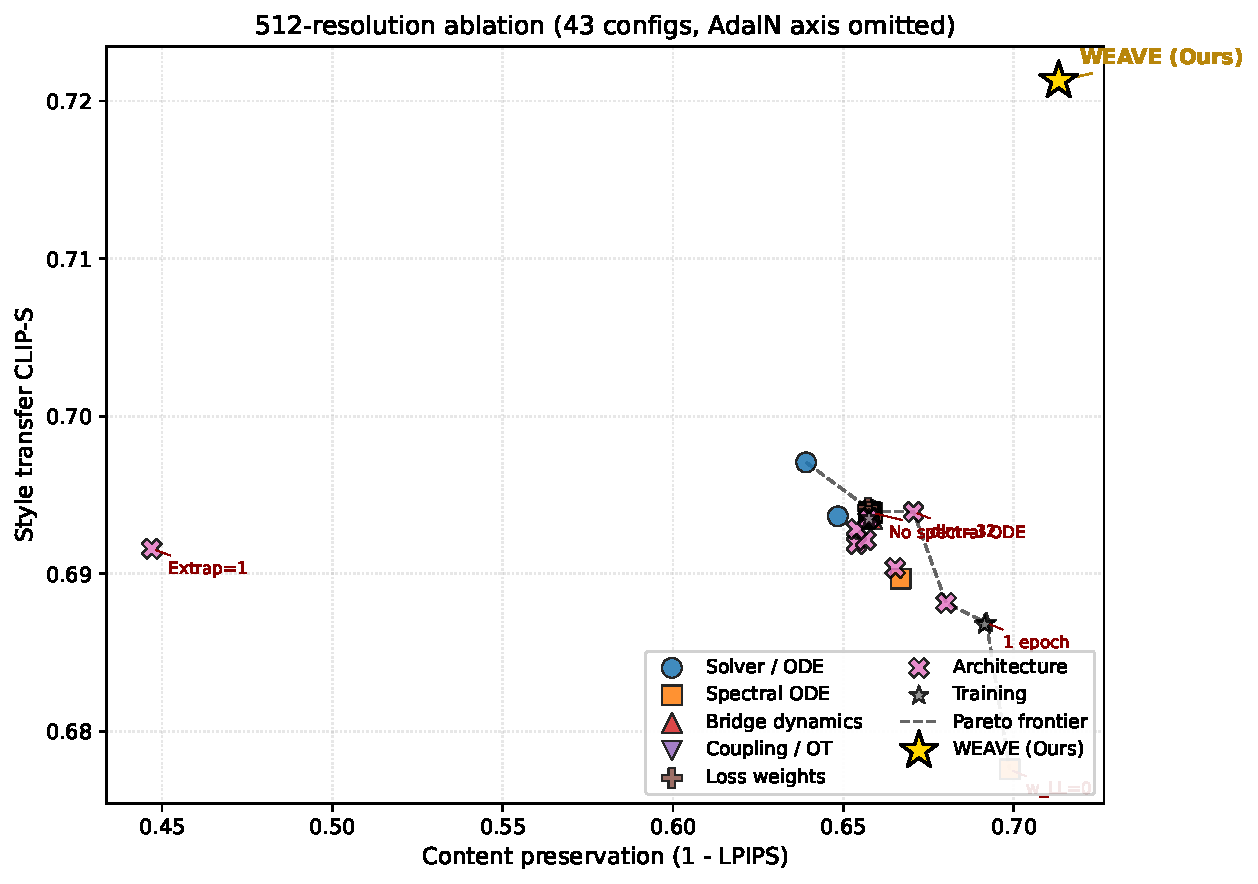
\includegraphics[width=0.85\linewidth]{fig_abl512_scatter.pdf}
\caption{512-resolution ablation scatter plot.
Each point is one of 48 ablation configurations, colored by theoretical axis; the gold star marks the full WD-VF model.
The dashed line is the Pareto frontier in the CLIP-S vs.\ $1{-}\mathrm{LPIPS}$ plane.
Three destructive clusters (AdaIN $4{\times}$, extrapolation~1, and LR~$10{\times}$) fall clearly off-frontier, validating the theoretical predictions.}
\label{fig:abl512_scatter}
\end{figure}

The scatter reveals a clear pattern.
Most configurations cluster tightly around the full model, demonstrating that the WD-VF design is robust to perturbations in solver order, path geometry, OT regularization, attention head count, and loss weights.
Three destructive clusters fall clearly off-frontier, and each matches a theoretical prediction.
Amplifying AdaIN ($4{\times}$) buys higher style score at the cost of catastrophic content damage, validating Proposition~\ref{prop:eota}: per-step style injection pushes the trajectory out of the correct-direction basin.
Setting the high-frequency extrapolation to~1 collapses content preservation, confirming that endpoint extrapolation is essential.
Increasing the learning rate by $10{\times}$ diverges to NaN, consistent with Theorem~\ref{thm:attractor}: the curvature condition requires the Adam step to stay below the wavelet-decoupled basin radius.
The Pareto frontier is traced by mild variants such as $w_{\mathrm{LL}}{=}0$ and $\mathrm{dim}{=}32$, confirming that low-frequency supervision and capacity reduction preserve content while leaving style transfer largely intact.
The wavelet coordinate change (Theorem~\ref{thm:attractor}), endpoint alignment (Proposition~\ref{prop:eota}), and the routing schedule are the three pieces carrying the result; the remaining axes are robust.

\subsection{Lightweight Few-Shot Generalization}

Beyond the main comparison, three controls test whether the result depends on representation, style vocabulary, and dataset bias.
All controls are reported on the full all-pairs protocol, consistent with the main table.

\paragraph{Latent prior carries the gain.}
A matched $256\times256$ control isolates whether the gain comes from wavelet transport in latent space or merely from adding another loss.
Direct RGB flow damages content far more than the latent-space control under the same protocol, confirming that the latent semantic prior, not the auxiliary loss, carries the result.

\paragraph{Few-shot style-memory update.}
Because WD-VF mathematically decouples the content structure (LL) from the style injection (LH/HL/HH), the learned high-frequency transport is not tied to a frozen five-style vocabulary.
We test this via a few-shot adaptation protocol: by exclusively updating the lightweight style-memory module using only a few reference images of a new style, the model preserves the correct-direction regime on an 8-style extension.
This confirms that WD-VF learns a generalizable mechanism for texture-and-stroke transport, rather than merely memorizing the training domains.

\paragraph{Random-20 generalization stress test.}
The Distinct5 benchmark is intentionally adversarial: the five target families were selected because they have the lowest identity CLIP-S, making accidental no-op success hardest.
A natural reviewer concern is therefore whether the result survives on a broader, non-cherry-picked style set.
We randomly sample 20 WikiArt families with at least 530 images each (Abstract Expressionism, Art Nouveau, Baroque, Color Field Painting, Cubism, Early Renaissance, Expressionism, Fauvism, High Renaissance, Impressionism, Mannerism, Minimalism, Na{\"\i}ve Art, Northern Renaissance, Pop Art, Post-Impressionism, Rococo, Romanticism, Symbolism, Ukiyo-e), train WD-VF from scratch with the same 5-epoch budget, and evaluate on 600 source-target pairs.
WD-VF retains the low-damage, correct-direction regime on this larger vocabulary, confirming that the Distinct5 result is not an artifact of the five selected styles.

Haar is not the only workable wavelet basis, but it is the most reliable default here.
Its exact orthogonality makes the subband decomposition literal.
Its local support keeps the supervision easy to interpret.
Daubechies-2 slightly raises CLIP-S but worsens LPIPS from 0.2868 to 0.3288.
We therefore keep Haar because it preserves the main CLIP-S/LPIPS tradeoff and keeps both the theory and the implementation simple.
On the current benchmark, we do not observe blocking artifacts that outweigh this tradeoff.

\section{Discussion}

\paragraph{Training efficiency.}
WD-VF trains in minutes because the objective is easier, not only because the network is small.
LL carries most global structure.
Once LL is weakly supervised and removed from the style-query path at inference, the model no longer spends most of its capacity on conflicting low-frequency objectives.
The remaining capacity can focus on high-frequency texture motion.

\paragraph{Mechanism of real style transfer.}
WD-VF edits the high-frequency subbands directly and aligns their endpoint statistics once, at the last step.
It does not repeatedly inject style through the whole trajectory.
This transfers stroke and surface texture while keeping the source layout stable.

\paragraph{Hard targets.}
Minimalism remains the hardest target family because its style change is driven more by low-frequency palette than by brushwork.
This matches the design.
LL is weakly supervised during transport and fixed during endpoint stylization.
WD-VF therefore favors structure stability over large palette shifts.

\paragraph{Limitations.}
WD-VF is domain-conditional rather than exemplar-conditional.
It is designed to reach a target style family, not to copy one reference painting.

The main benchmark is intentionally narrow.
It isolates five hard WikiArt styles chosen by low IDT CLIP-S.
This makes it a focused stress test for no-op failure rather than a full account of cross-domain or open-vocabulary stylization.
IDT should therefore be read as a calibration protocol for this art-to-art setting.
The Random-20 experiment partially addresses this concern by showing that the same low-damage, correct-direction regime survives on a larger, non-cherry-picked style vocabulary.

The LL design makes palette-heavy targets such as Minimalism harder than heavily textured targets.
The method deliberately protects low-frequency structure.
Large palette shifts are therefore less favored than brushwork and surface-texture changes.

The theory is local and mechanism-oriented.
It explains one failure mode of Euclidean latent flow and predicts the related ablations.
It does not address global convergence or every possible collapse mechanism.

The current main table is single-seed and benchmark-specific.
The effect sizes are large, but broader multi-seed evaluation would strengthen the empirical case.
Broader cross-domain data would also test whether the same IDT-calibrated story survives outside WikiArt-to-WikiArt transfer.

\section{Conclusion}

Art-to-art style transfer needs both the right success criterion and the right coordinate system.
IDT calibration exposes when a method is only reconstructing the source.
WD-VF avoids this regime by separating low-frequency structure from high-frequency style motion and by routing style through the same high-frequency path used at inference.
On Distinct5-WikiArt, it reaches CLIP-S/LPIPS of 0.7213/0.2868 with 903K trainable parameters in its flow backbone.
Training takes 3.08 minutes on a single RTX 3060.
Generation plus VAE decode takes 83.7 seconds for 750 outputs.
The theory explains one Euclidean failure mode and predicts the ablation pattern confirmed by experiment.
While trained on a focused benchmark, the decoupled nature of WD-VF allows for rapid, few-shot extension to new styles without altering the base network, and the same low-damage, correct-direction regime survives on a Random-20 generalization split (0.7434 CLIP-S / 0.2910 LPIPS), offering a highly sustainable paradigm for generative style editing.
The main result is simple: real target-direction transfer does not require a large model if the transport geometry separates structure from style.

\section*{Ethics Statement}
Style transfer tools can be misused to produce deceptive images or to misattribute stylistic authorship.
Our method operates at the domain level (e.g., ``Impressionism'') rather than the per-artist level.
This reduces the risk of imitating a specific living artist.
We do not condition on individual reference paintings.
The dataset is sourced from WikiArt and contains historically significant artworks.
It does not contain personal data.
We encourage downstream users to disclose when an image has been style-transferred and to respect source-content licensing terms.

\section*{Reproducibility Statement}
All experiments use public data (WikiArt) and a public VAE (Stable Diffusion v1.5 EMA VAE).
Section~\ref{sec:exp} gives the training configuration, hyperparameters, and evaluation protocol.
Training takes 3.08 minutes on a single RTX 3060 (12\,GB).
The 750-pair evaluation run needs 83.7 seconds for generation plus VAE decode and 97.3 seconds including CLIP/LPIPS metrics.
The 903K trainable parameter backbone checkpoint is 3.5\,MB.
We will release the code, the checkpoint, and the 750-pair evaluation protocol upon publication.

\FloatBarrier

\bibliography{refs}

\section*{AAAI Reproducibility Checklist}

\begin{enumerate}
\item This paper claims the following contributions:
(1)~IDT-calibrated evaluation for art-to-art transfer (Section~\ref{sec:exp});
(2)~analysis of Euclidean collapse through the set $\mathcal{M}_0$ and Theorem~\ref{thm:attractor} (Section~\ref{sec:attractor});
(3)~the WD-VF method, a wavelet-decoupled rectified flow with high-frequency query routing and endpoint subband alignment (Section~\ref{sec:method});
(4)~objective decomposition in the high-frequency-only query case and its ablation-level consequences (Section~\ref{sec:opt}).
\item The dataset (Distinct5-WikiArt-512) is publicly available. The evaluation protocol (CLIP-S, LPIPS, 750 pairs including 150 identity pairs) is described in Section~\ref{sec:exp}.
\item Code, checkpoint, and evaluation scripts will be released upon publication.
\item Training requires a single 12\,GB GPU (RTX 3060); 5 epochs; 3.08 minutes end-to-end.
\item The evaluation protocol uses HuggingFace CLIP ViT-B/32 and AlexNet LPIPS, with 750 (source, target) pairs across 5 domains.
\item All baseline numbers (Table~\ref{tab:main}) are evaluated under the same protocol.
SaMST and SaMam have explicit convergence records.
CUT uses an archived checkpoint with recorded training time but no surviving training log.
\item Statistical reporting: Table~\ref{tab:main} reports the main single-seed 750-pair results.
The supplement provides ablations, boundary-case analyses, and extension studies.
\end{enumerate}

\end{document}
